\documentclass[letter,12pt]{article}
\usepackage{fontenc}
\usepackage[english]{babel}

\usepackage{fullpage}
\usepackage{amsmath,amssymb}
\usepackage[colorlinks=true,linkcolor=blue,citecolor=blue]{hyperref}
\bibliographystyle{plain}

\usepackage[pdftex]{graphicx}
\usepackage{epstopdf}
\epstopdfsetup{outdir=./IMAGES/}
\graphicspath{ {IMAGES/} }

\title{The temperature-size rule is predicted to stabilise consumer-resource dynamics under warming}
\date{\today}
\author{UBC MST group}

\begin{document}
\maketitle
\tableofcontents

%%%%%%%%%%%%%%%%%%%%%%%%%%%%%%%%%%%%%%%%%%%%%%%%%%%%%%%
\section*{Abstract}
%%%%%%%%%%%%%%%%%%%%%%%%%%%%%%%%%%%%%%%%%%%%%%%%%%%%%%%

%%%%%%%%%%%%%%%%%%%%%%%%%%%%%%%%%%%%%%%%%%%%%%%%%%%%%%%
\textbf{Keywords:} Metabolic theory, predator-prey, plant-herbivore, body size
%%%%%%%%%%%%%%%%%%%%%%%%%%%%%%%%%%%%%%%%%%%%%%%%%%%%%%%

%%%%%%%%%%%%%%%%%%%%%%%%%%%%%%%%%%%%%%%%%%%%%%%%%%%%%%%
\section{Introduction}
%%%%%%%%%%%%%%%%%%%%%%%%%%%%%%%%%%%%%%%%%%%%%%%%%%%%%%%

Temperature and body size determine many biological rates \cite{West1997,Gillooly2001}.
How these factors individually influence consumer-resource dynamics has already been demonstrated \cite{Gilbert2014,DeLong2015}.
How they act in symphony has not yet been investigated.

Temperature also affects body size through the temperature-size rule \cite{Atkinson1994}.
Thus, temperature directly and indirectly affects ecosystem dynamics.
These two pathways have the potential to reinforce or counteract one another, with population level consequences.

Here we model a simple consumer-resource interaction, with population dynamic parameters that depend on temperature and body size, and body sizes that depend on temperature.
We ask how including dependencies on both temperature and body size, as well as incorporating the temperature-size rule, affects the response of the consumer-resource dynamics to increasing temperature.

%%%%%%%%%%%%%%%%%%%%%%%%%%%%%%%%%%%%%%%%%%%%%%%%%%%%%%%
\section{Methods and results}
%%%%%%%%%%%%%%%%%%%%%%%%%%%%%%%%%%%%%%%%%%%%%%%%%%%%%%%

%%%%%%%%%%%%%%%%%%%%%%%%%%%
\subsection{The underlying consumer-resource dynamics}

We begin, like \cite{Gilbert2014}, with the Rosenzweig-MacArthur equations \cite{Rosenzweig1963}
\begin{equation}\label{eq:RM}
\begin{aligned}
\frac{\mathrm{d}R}{\mathrm{d}t} =& r R \left(1 - \frac{R}{K} \right) - f(R) C\\
\frac{\mathrm{d}C}{\mathrm{d}t} =& e f(R) C - m C,
\end{aligned}
\end{equation}
which describe the rates of change in total resource $R\in[0,K]$ and consumer $C\geq0$ biomass with time $t$.

In the absence of consumers, $C=0$, the resource grows logistically, with intrinsic growth rate $r\geq0$ and carrying capacity $K>0$.
The intrinsic growth rate describes the rate at which resource biomass increases without consumers when the resource is rare, $R\approx0$.
The carrying capacity is the equilibrium biomass of the resource without consumers.

Resource biomass is consumed by consumers at a rate $f(R)$, where $f(R)\geq0$ is called the functional response.
Of the biomass consumed, the unitless conversion efficiency parameter $e\in[0,1]$ determines the proportion of resource biomass that is directly converted into consumer biomass.
Consumers die at constant per capita mortality rate $m\geq0$.

An equilibrium is reached when the two rates of change in Equation \eqref{eq:RM} are zero, and solving the system at this point gives equilibrium resource $\hat{R}$ and consumer $\hat{C}$ biomass.
There are three equilibria for this system: total extinction $(R,C) = (0,0)$, consumer extinction $(R,C)=(K,0)$, and coexistence $(R,C)=(\hat{R},\hat{C})$, the latter with $\hat{R}>0$ and $\hat{C}>0$.
We are primarily concerned with the latter equilibrium, as that is presumably the equilibrium current consumer-resource systems are near.
At this coexistence equilibrium one can calculate the ratio of consumer to resource biomass, $\hat{C}:\hat{R}$, and also perform a linear stability analysis to derive the leading (largest in absolute value) eigenvalue $\lambda$, which determines if (and how readily) the system, when perturbed a small amount from this equilibrium, will return to it (see the supplementary \texttt{Mathematica} file for details).
Our measure of stability will be the negative of the real part of the leading eigenvalue.
The system is stable if and only if this value is positive, and the system will return to equilibrium faster when this value is larger (i.e., larger positive values imply ``more stable" systems).
Together these two measures tell us how biomass is partitioned and how stable this partitioning is.

As explained in \cite{Gilbert2014}, two aggregates well describe the dynamics of this system.
The first is $m R/(e f(R))$, which describes consumer growth and is the consumer zero-net growth isocline.
The second aggregate is $K$, the equilibrium resource biomass in the absence of consumers.
Dividing the second aggregate by the first gives a measure that defines the biomass potential of the resource that is converted into consumer biomass, $B_{CR} = e f(R) K / (R m)$.
Note that we have modified the presentation of \cite{Gilbert2014} by subsuming $R$ into $f(R)$ such that $f(R)$ is  a rate and thus more easily interpreted.
This does not alter the results.

In what follows we will examine how our three measures, $B_{CR}$, $\hat{C}:\hat{R}$, and stability, change with temperature.
We start by assuming a type-I functional response, $f(R) = a R$, where $a$ is called the attack rate, which describes the rate of resource consumption per resource biomass.
We later explore the effect of a type-II functional response and the potential for the functional response to change with temperature.

%%%%%%%%%%%%%%%%%%%%%%%%%%%
\subsection{Temperature dependence}

Gilbert \textit{et al.} \cite{Gilbert2014} discuss what is known about the temperature dependencies of $r$, $K$, $a$, $m$, and $e$, and give equations and parameter estimates in their Table 1.
Briefly, resource growth rate $r$ is expected to scale with metabolism as a Boltzmann-Arrhenius factor, $r(T) = r_0 \exp(-E_B/(kT))$, where $E_B$ is the activation energy of the metabolism $B$ (in units of eV), $k$ is Boltzmann's constant ($\approx 8.62 \times 10^{-5}$ eV/K), and $T$ is the temperature (in Kelvins).
Resource carrying capacity $K$ is determined by the ratio of the supply rate of nutrients into the system and the rate of uptake of nutrients by the resource, $r$.
With supply rate also scaling as a Boltzmann-Arrhenius factor with activation energy $E_S$, carrying capacity is  $K(T) = K_0 \exp(-(E_S - E_B)/(kT))$. 
Attack rate $a$ depends on the temperature dependence of the body velocities $\nu$ in both species, which both scale as Boltzmann-Arrhenius factors with activation energies $E_{\nu,i}$, with $i=\{R,C\}$.
Attack rate is then $a(T) = a_0 \sqrt{\sum \left[\nu_{0,i} \exp(-E_{\nu,i}/(kT)) \right]^2}$, where the sum is over $i=\{R,C\}$ and $\nu_{0,i}$ are rate-constants.
Consumer mortality is also expected to scale as a Boltzmann-Arrhenius factor, $m(T) = m_0 \exp(-E_m/(kT))$.
Conversion efficiency is assumed to be independent of temperature $e(T) = e_0$.

Figure \ref{AllTempDep} shows $B_{CR}$, equilibrium consumer to resource biomass ratio $\hat{C}:\hat{R}$, and stability of the coexistence equilibrium as functions of temperature $T$ (plotted in Celsius).
In these plots $r$, $K$, $a$, and $m$ all depend on temperature as discussed above, unlike Figure 3 in \cite{Gilbert2014} where only $K$ depends on temperature and the rest of the parameters are held constant.
Comparing with Figure 3 in \cite{Gilbert2014} shows that adding temperature dependence in $r$, $a$, and $m$ causes consumer:resource biomass to decline with temperature (instead of increasing) and stability to decrease at a slower rate  with increasing temperature.
These changes are largely driven by the temperature dependence of consumer mortality: increasing temperature increases consumer mortality, lowering its equilibrium biomass and increasing stability at high temperatures (relative to the case where $m$ does not depend on temperature).

\begin{figure}[!ht]
\centering
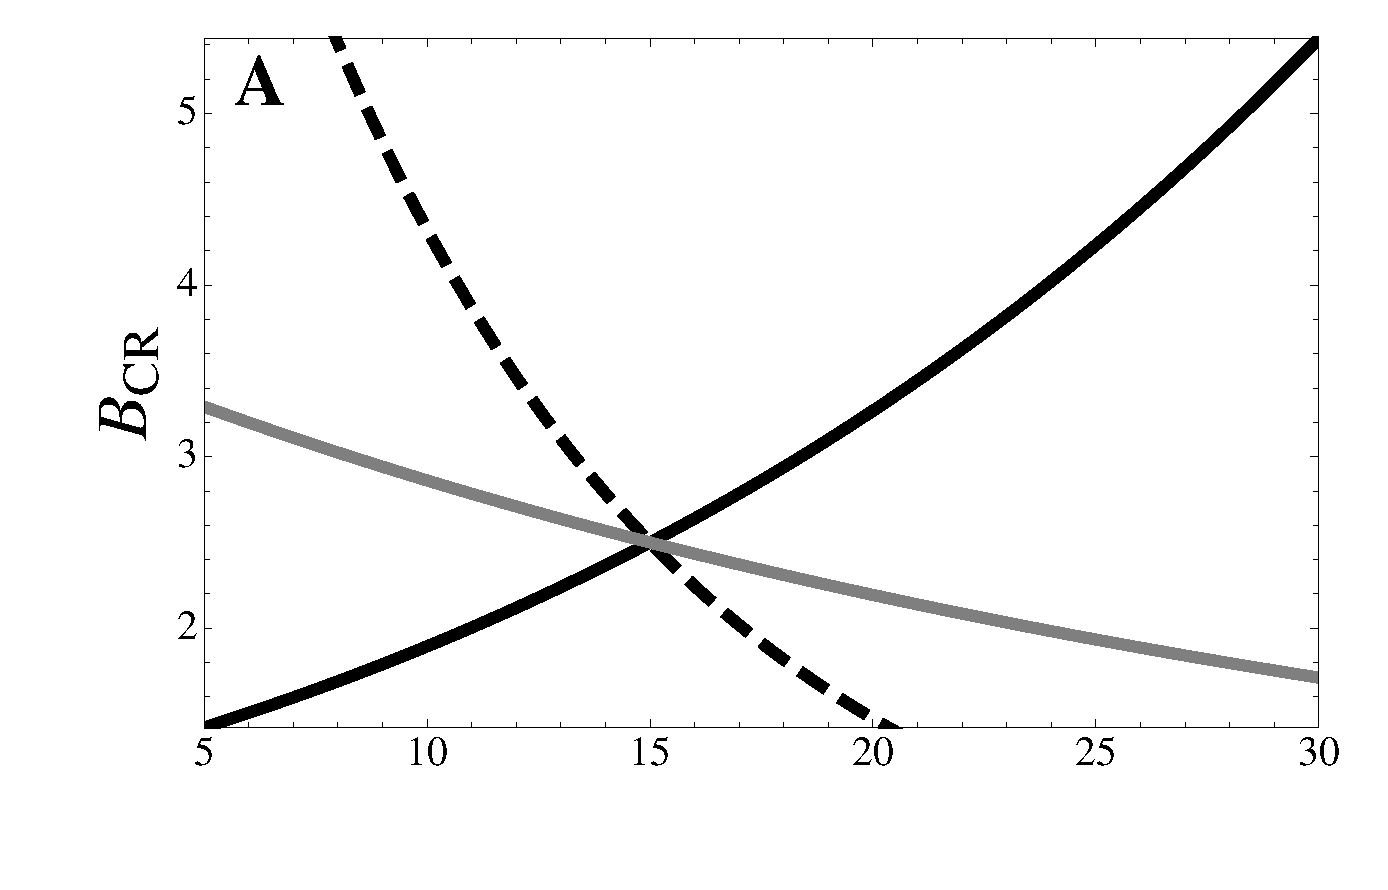
\includegraphics[width=0.5\linewidth]{BCRAllTempDep}
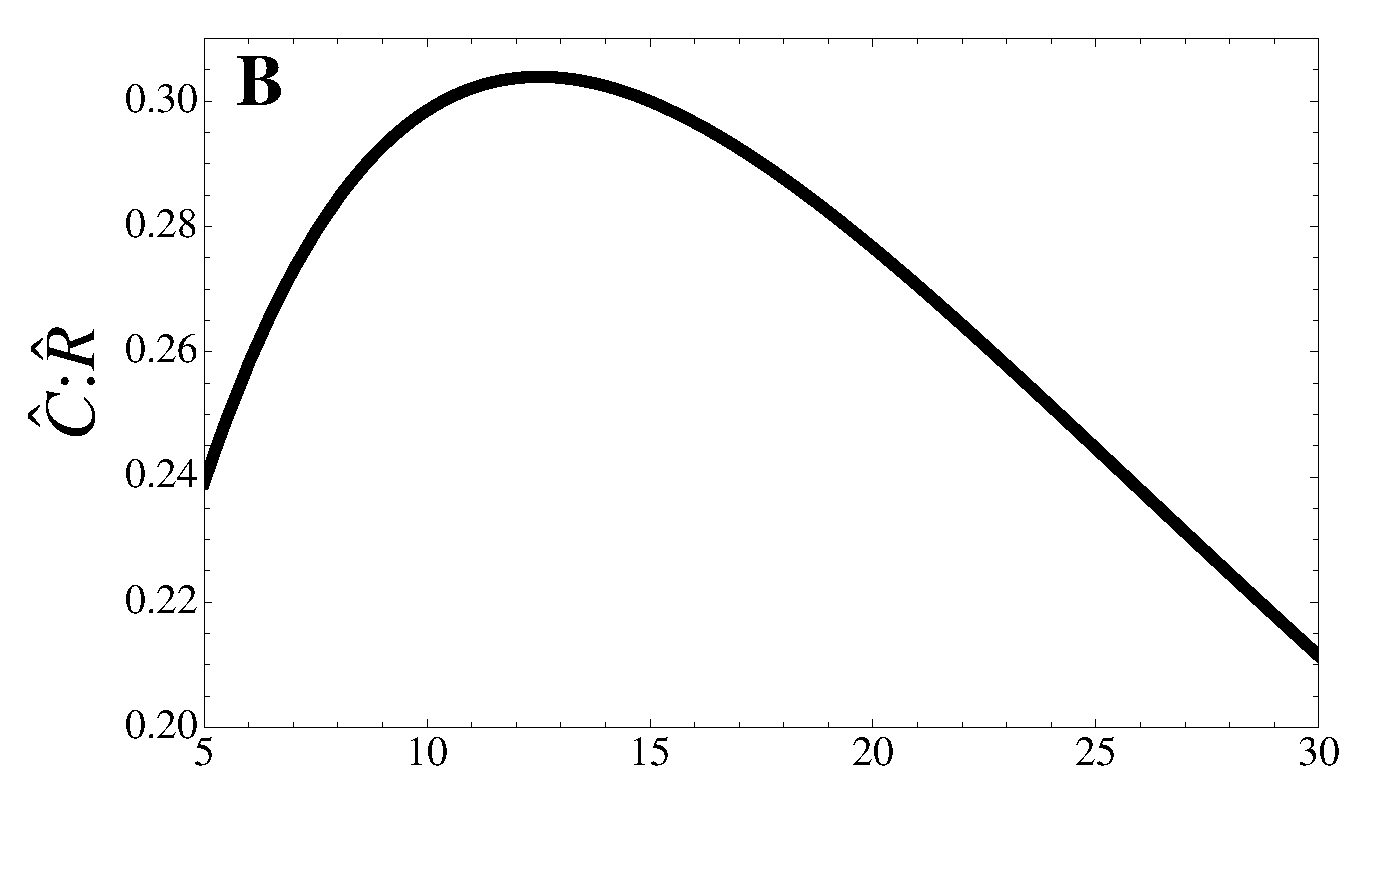
\includegraphics[width=0.5\linewidth]{CtoRAllTempDep}
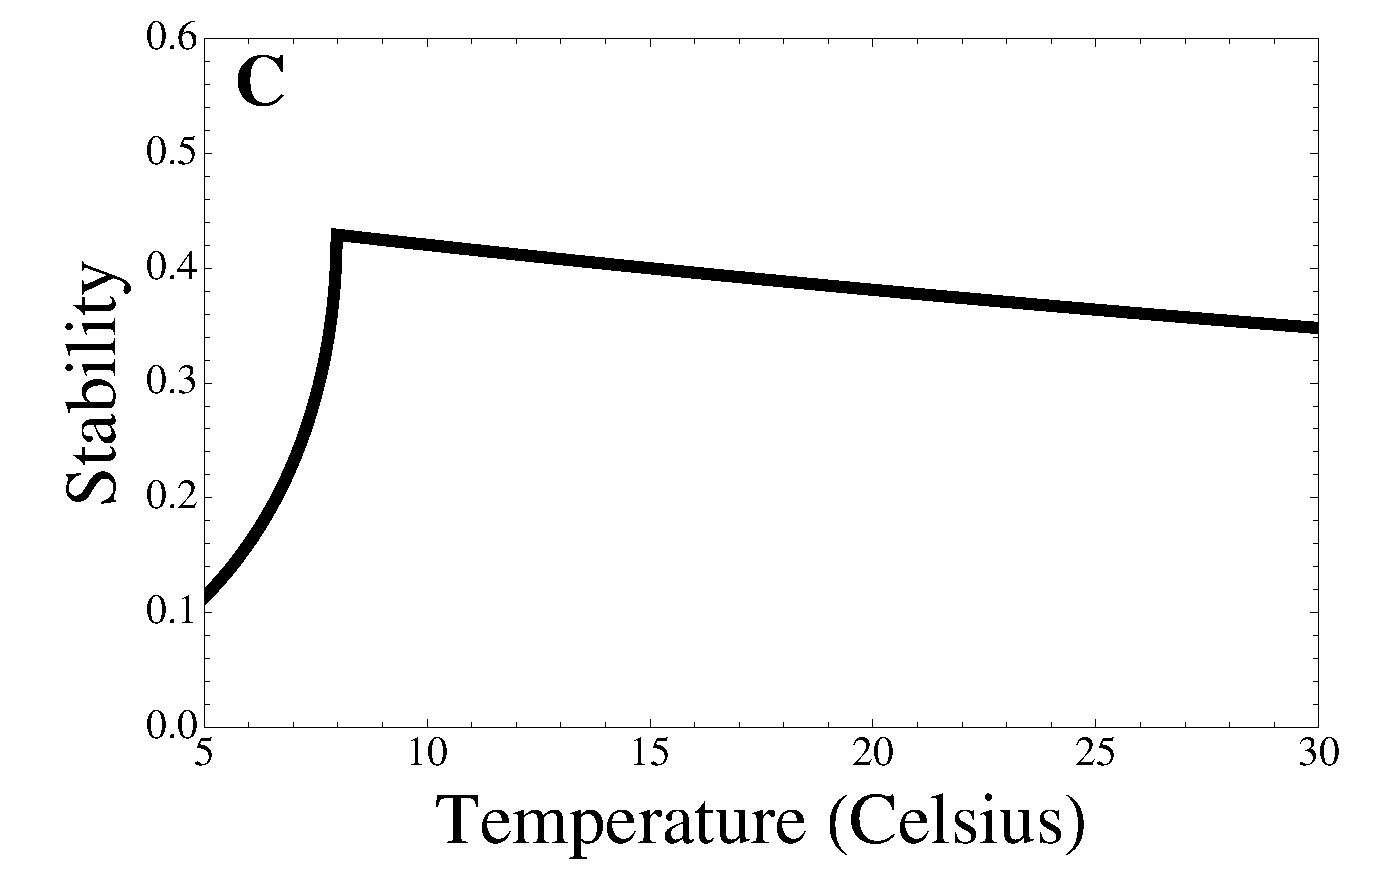
\includegraphics[width=0.5\linewidth]{StabilityAllTempDep}
\caption{
$B_{CR}$, equilibrium consumer to resource biomass ratio $\hat{C}:\hat{R}$, and stability of the coexistence equilibrium as functions of temperature $T$ (plotted in Celsius).
Rate-constants (e.g., $r_0$) were chosen to make $r = 2$, $K = 100$, $a = 0.1$, $m = 0.6$, and $e = 0.15$ at 15$^\circ C$ (as in \cite{Gilbert2014}).
Other parameters: $E_B = 0.32$ (solid black), $E_B = 0.9$ (dashed and gray), $E_S = 0.9$ (solid black and gray), $E_S = 0.32$ (dashed), $E_m = 0.65$, $E_{\nu,i} = 0.46$, $\nu_{0,i} = 1$.  
}
\label{AllTempDep}
\end{figure}


%%%%%%%%%%%%%%%%%%%%%%%%%%%
\subsection{Mass dependence and the temperature size-rule}

We next allow the population dynamic parameters to depend on the body mass of resource and consumer.
Following \cite{DeLong2015}, each parameter can be written as a power law function of resource or consumer body size.
To let the parameters depend on both temperature and mass we multiply each by the power-law mass dependence, giving: $r(T, M_R) = r(T) M_R^\rho$, $K(T, M_R) = k(T) M_R^\kappa$, $a(T, M_C) = a(T) M_C^\alpha$, $e(T, M_C) = e(T) M_C^\epsilon$, and $m(T, M_C) = m(T) M_C^\mu$.

If mass does not change with temperature then adding these mass dependencies does not change the response of the consumer-resource dynamics to temperature.
However, mass is expected to change with temperature, according to the temperature-size rule \cite{Atkinson1994}.
%For organisms with a dry mass of less than $10^{-3}$ mg body mass declines linearly with temperature.
We incorporate a simple form of the temperature-size rule here for illustrative purposes.
In particular, we assume mass declines linearly with temperature, $M_i(T) = M_i(T_{ref}) (1 - \beta_i (T - T_{ref})$, where $\beta_i$ is the fraction that mass is reduced as temperature is increased by one degree and $T_{ref}$ is a reference temperature, which we set to 15$^\circ C$ throughout.
This linear decline best approximates the response of organisms with a dry mass of less than $10^{-3}$ mg \cite{Forster2012}.
Larger organisms experience a faster than linear decline.

Figure \ref{AllTempMassDep} is our main result, which shows how adding mass dependencies and the temperature-size rule modifies our prediction of how consumer-resource dynamics respond to changes in temperature.
While there is little change in $B_{CR}$ in Figure \ref{AllTempMassDep}, the consumer to resource biomass ratio is no longer expected to decline with increasing temperature and stability is expected to increase.
These changes are brought on by the indirect effect of temperature, through mass, on the population dynamic parameters.
In particular, the lack of decline in the consumer to resource biomass ratio with the temperature-size rule, relative to the case without it, seems to be primarily driven by changes in consumer conversion efficiency and the intrinsic growth rate of the resource.
Both of these rates increase with declining body mass, supporting a larger biomass of consumers. 
The result of these indirect effects acts in opposition to the direct effect of temperature, and in the case of stability overrides the direct effect to produce a qualitatively different prediction.
%The increase in stability with the temperature-size rule stimulates the tantalizing possibility that its existence is adaptive, although obviously much more careful thought is needed here.

\begin{figure}[!ht]
\centering
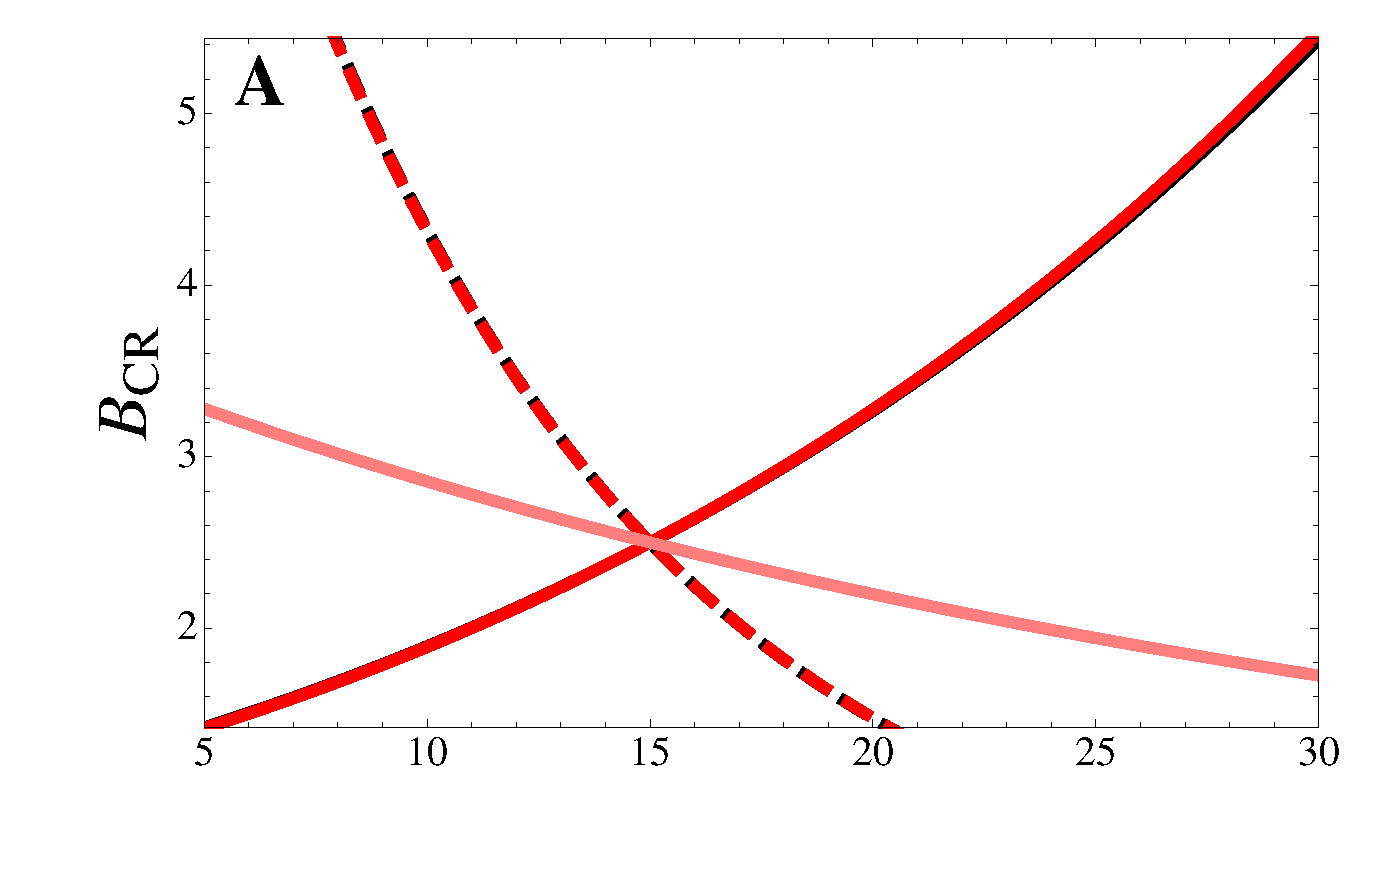
\includegraphics[width=0.5\linewidth]{BCRAllTempMassDep}
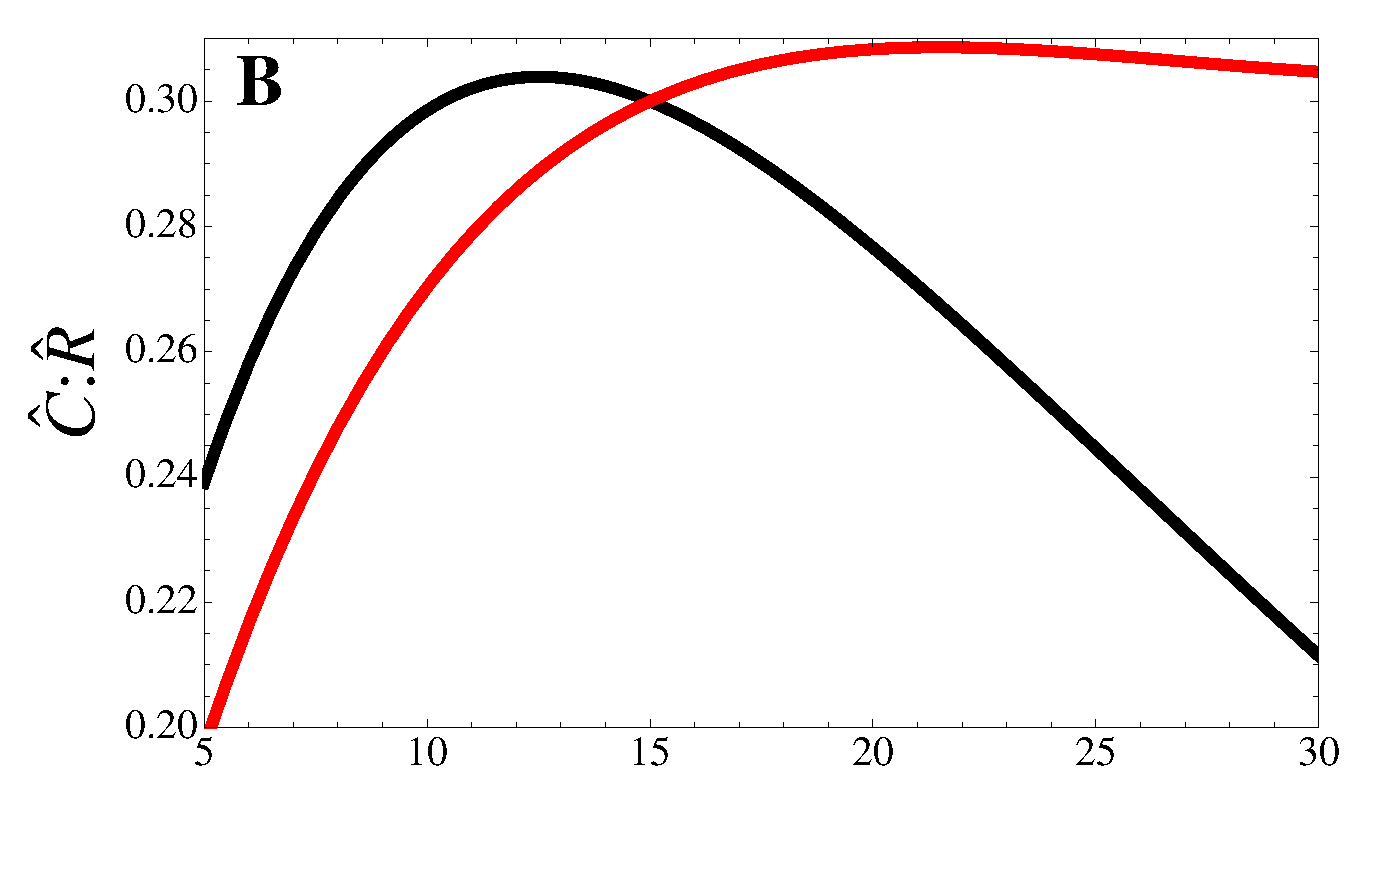
\includegraphics[width=0.5\linewidth]{CtoRAllTempMassDep}
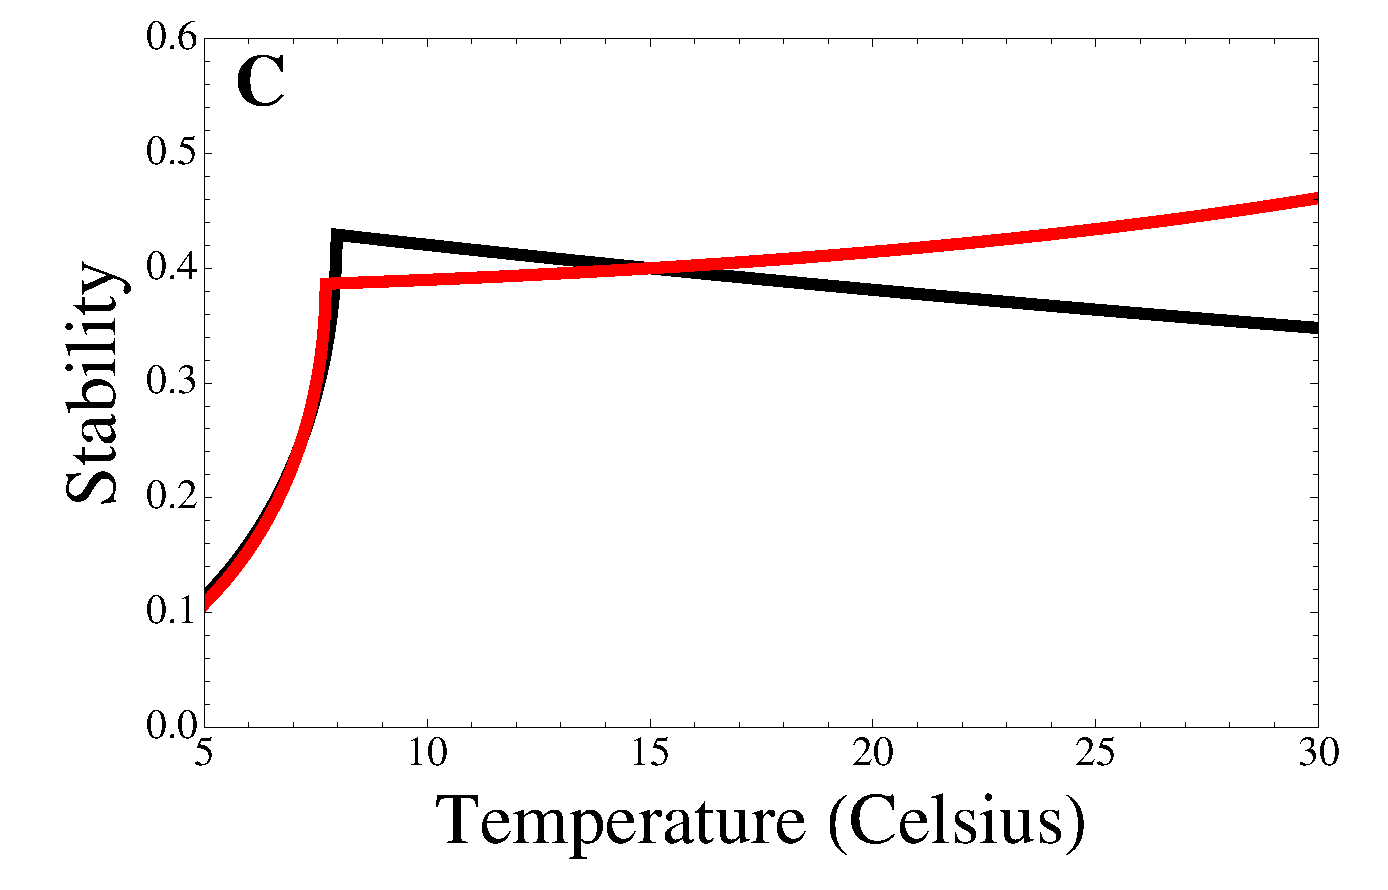
\includegraphics[width=0.5\linewidth]{StabilityAllTempMassDep}
\caption{
$B_{CR}$, equilibrium consumer to resource biomass ratio $\hat{C}:\hat{R}$, and stability of the coexistence equilibrium as functions of temperature $T$ (plotted in Celsius) with (red) and without (black) mass dependencies and the temperature-size rule.
Rate-constants (e.g., $r_0$) were chosen to make $r = 2$, $K = 100$, $a = 0.1$, $m = 0.6$, and $e = 0.15$ at 15$^\circ C$ (as in \cite{Gilbert2014}).
Other parameters as in \cite{Gilbert2014,DeLong2015}: $E_B = 0.32$ (solid dark), $E_B = 0.9$ (dashed and solid light), $E_S = 0.9$ (solid), $E_S = 0.32$ (dashed), $E_m = 0.65$, $E_{\nu,i} = 0.46$, $\nu_{0,i} = 1$, $\kappa = -0.81$, $\alpha = 1$, $\epsilon = -0.5$, $\mu = -0.29$, $\rho = -0.81$, $\beta_i = 0.02$ (red), $\beta_i = 0$ (black).  
}
\label{AllTempMassDep}
\end{figure}

%%%%%%%%%%%%%%%%%%%%%%%%%%%
\subsection{Asymmetric temperature-size responses}

In Figure \ref{AllTempMassDep} we assumed both resource and consumer body mass declined with temperature at the same rate, $\beta_C = \beta_R = 0.02$, i.e., both decline $2\%$ per degree increase.
However, it has been shown that larger organisms experience larger declines in body size with temperature \cite{Forster2012}.
In Figure \ref{AllTempMassDepAsymm} we let consumer body size decline twice as fast as the resource, $2 \beta_R = \beta_C = 0.04$.
In this case our results are in even greater disagreement with \cite{Gilbert2014}, and increases in temperature now increases stability to a greater extent.

\begin{figure}[!ht]
\centering
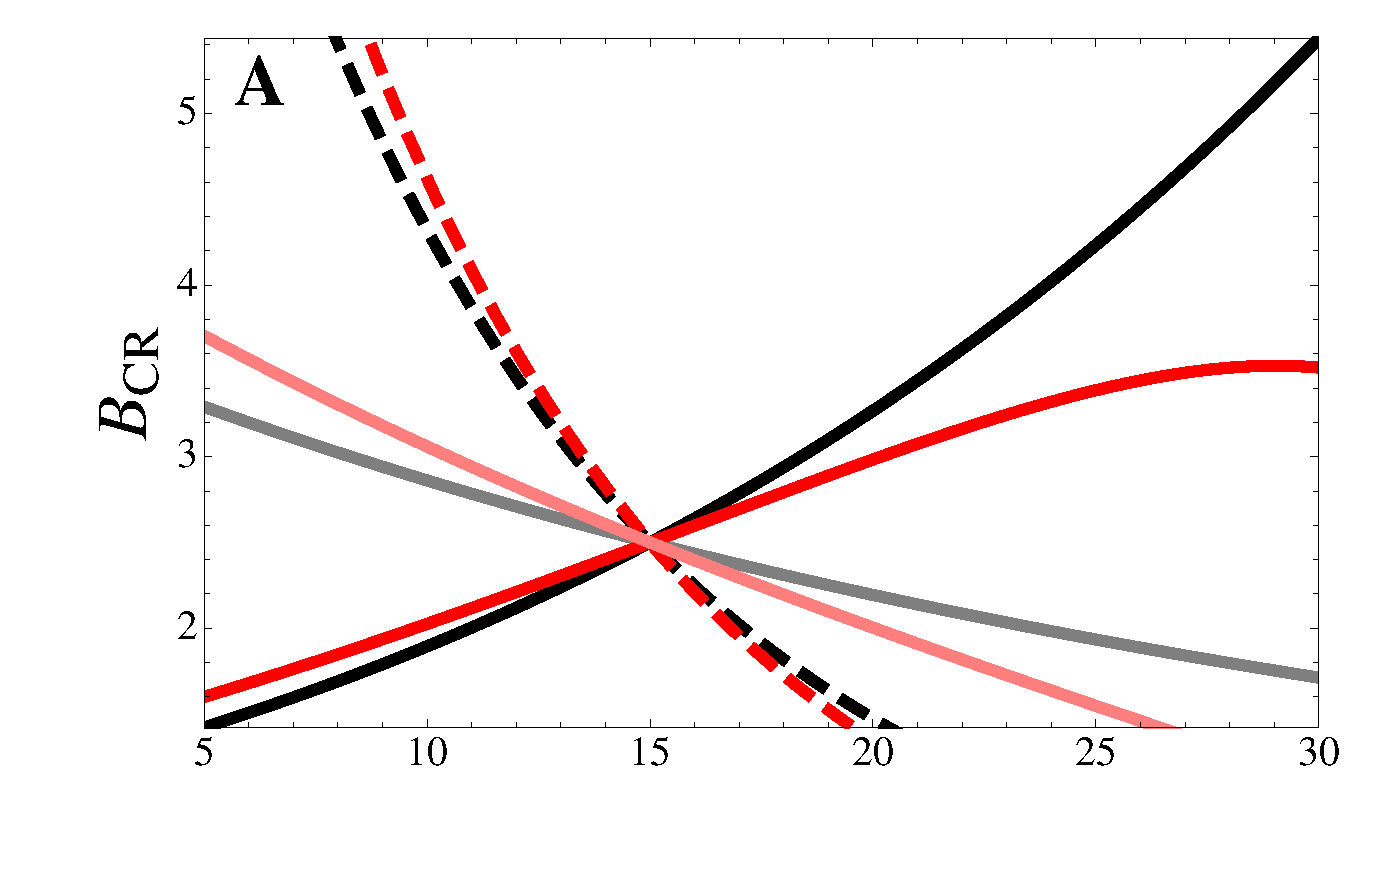
\includegraphics[width=0.5\linewidth]{BCRAllTempMassDepAsymm}
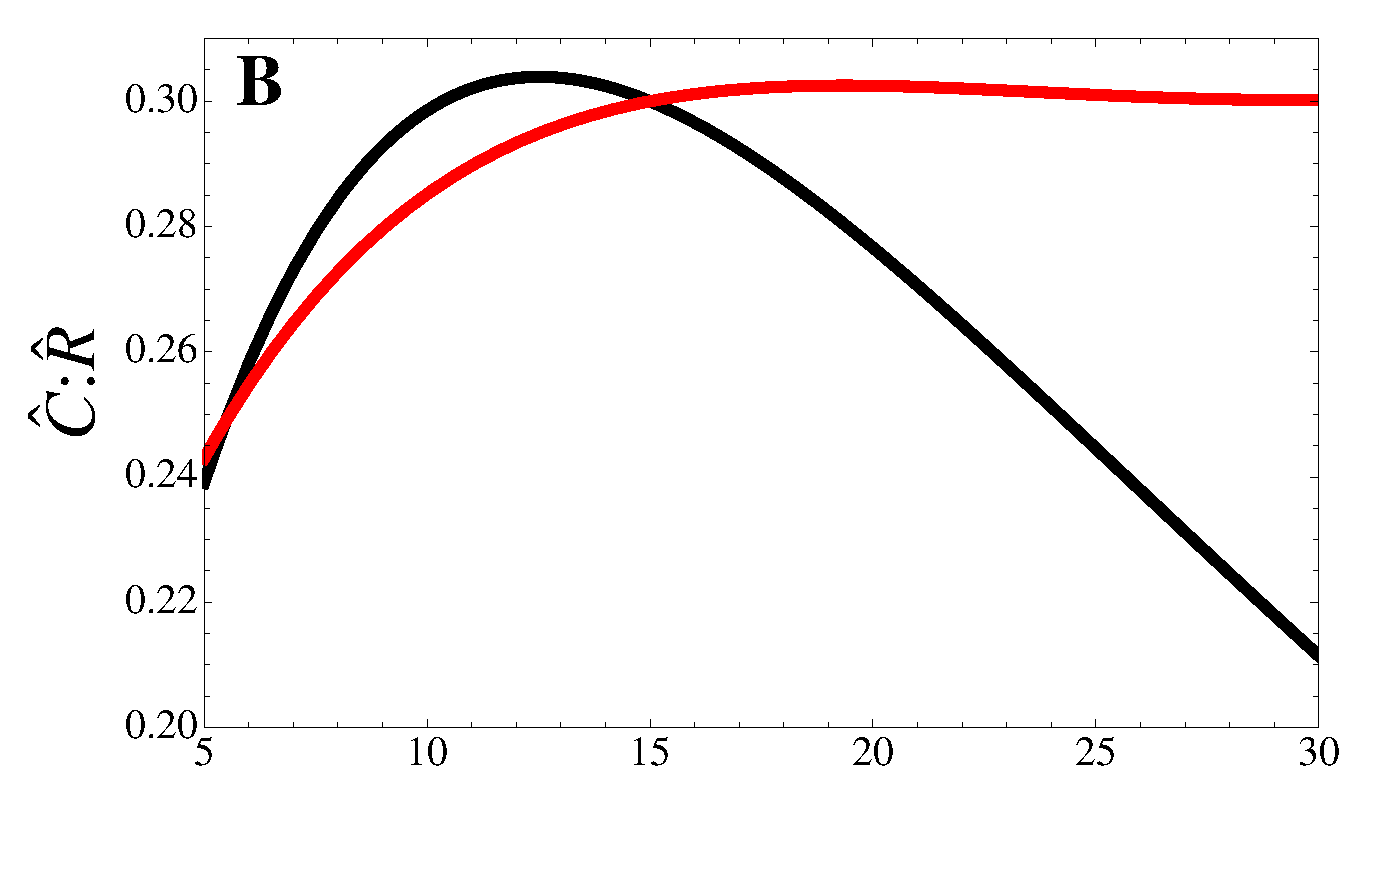
\includegraphics[width=0.5\linewidth]{CtoRAllTempMassDepAsymm}
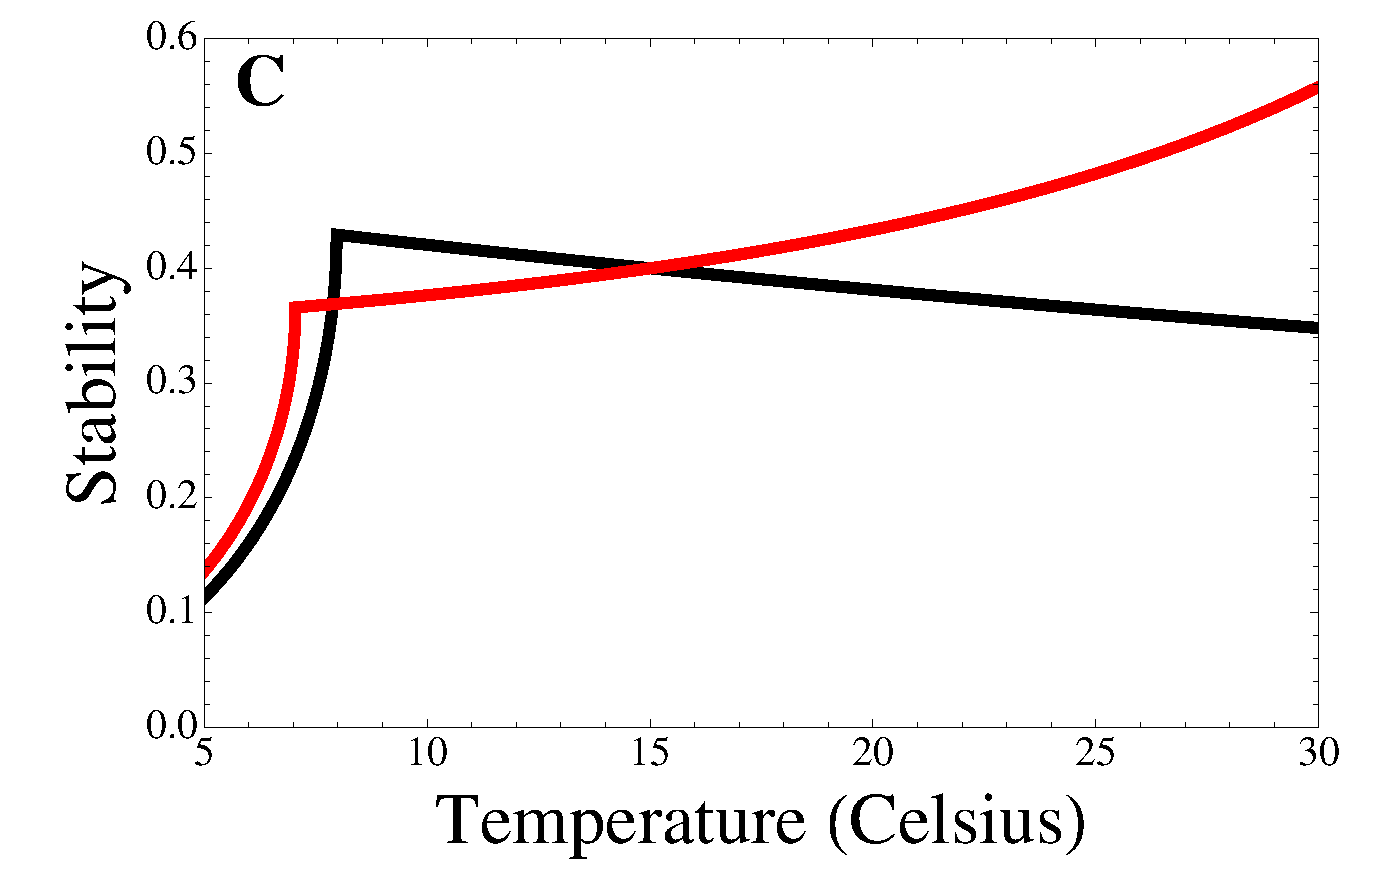
\includegraphics[width=0.5\linewidth]{StabilityAllTempMassDepAsymm}
\caption{
$B_{CR}$, equilibrium consumer to resource biomass ratio $\hat{C}:\hat{R}$, and stability of the coexistence equilibrium as functions of temperature $T$ (plotted in Celsius) with (red) and without (black) mass dependencies and the temperature-size rule.
Rate-constants (e.g., $r_0$) were chosen to make $r = 2$, $K = 100$, $a = 0.1$, $m = 0.6$, and $e = 0.15$ at 15$^\circ C$ (as in \cite{Gilbert2014}).
Other parameters as in \cite{Gilbert2014,DeLong2015}: $E_B = 0.32$ (solid dark), $E_B = 0.9$ (dashed and solid light), $E_S = 0.9$ (solid), $E_S = 0.32$ (dashed), $E_m = 0.65$, $E_{\nu,i} = 0.46$, $\nu_{0,i} = 1$, $\kappa = -0.81$, $\alpha = 1$, $\epsilon = -0.5$, $\mu = -0.29$, $\rho = -0.81$, $\beta_R = 0.02$ and $\beta_C = 0.04$ (red), $\beta_i = 0$ (black).  
}
\label{AllTempMassDepAsymm}
\end{figure}

%%%%%%%%%%%%%%%%%%%%%%%%%%%
\subsection{Type-II functional response}

The consumption of resources in many systems is better described by a type-II functional response, which is linear in resource biomass at low resource biomass (like the type-I functional response) but asymptotes at higher resource biomass, describing satiation of the consumer.

%%%%%%%%%%%%%%%%%%%%%%%%%%%%%%%%%%%%%%%%%%%%%%%%%%%%%%%
\section{Discussion}
%%%%%%%%%%%%%%%%%%%%%%%%%%%%%%%%%%%%%%%%%%%%%%%%%%%%%%%

%%%%%%%%%%%%%%%%%%%%%%%%%%%%%%%%%%%%%%%%%%%%%%%%%%%%%%%
\bibliography{BIB/library}

\end{document}
